\documentclass[a4paper,12pt]{report}
\usepackage[toc,page]{appendix}
\usepackage{amsmath}
\usepackage{float}
\usepackage{graphicx}
\usepackage{subfig}
\usepackage{geometry}
\usepackage{array}
\usepackage{tcolorbox}
\usepackage[normalem]{ulem}
\usepackage{amsmath,amsfonts,amssymb}
\usepackage{multicol}
\usepackage{color}
\usepackage{listings}
\usepackage{setspace}
\usepackage{arydshln}

\usepackage{setspace}
 \geometry{
 a4paper,
 total={170mm,257mm},
 left=20mm,
 top=20mm,
 }

\usepackage{listings}
\usepackage{mathtools}
% Python style for highlighting
\newcommand\pythonstyle{\lstset{
language=Python,
basicstyle=\ttm,
otherkeywords={self},             % Add keywords here
keywordstyle=\ttb\color{deepblue},
emph={MyClass,__init__},          % Custom highlighting
emphstyle=\ttb\color{deepred},    % Custom highlighting style
stringstyle=\color{deepgreen},
frame=tb,                         % Any extra options here
showstringspaces=false            % 
}}


% Python environment
\lstnewenvironment{python}[1][]
{
\pythonstyle
\lstset{#1}
}
{}

% Python for external files
\newcommand\pythonexternal[2][]{{
\pythonstyle
\lstinputlisting[#1]{#2}}}

% Python for inline
\newcommand\pythoninline[1]{{\pythonstyle\lstinline!#1!}}
\usepackage{graphicx}
\usepackage{tikz,tikz-3dplot, esvect}
\usetikzlibrary{calc,3d,arrows,shapes}

\usepackage{verbatim}
\begin{document}

\title{Project 2 of Robotics Nanodegree \\
Pick and Place,  \\
Kuka KR210: a 6DOF manipulator
\begin{figure}[H]
\centering
        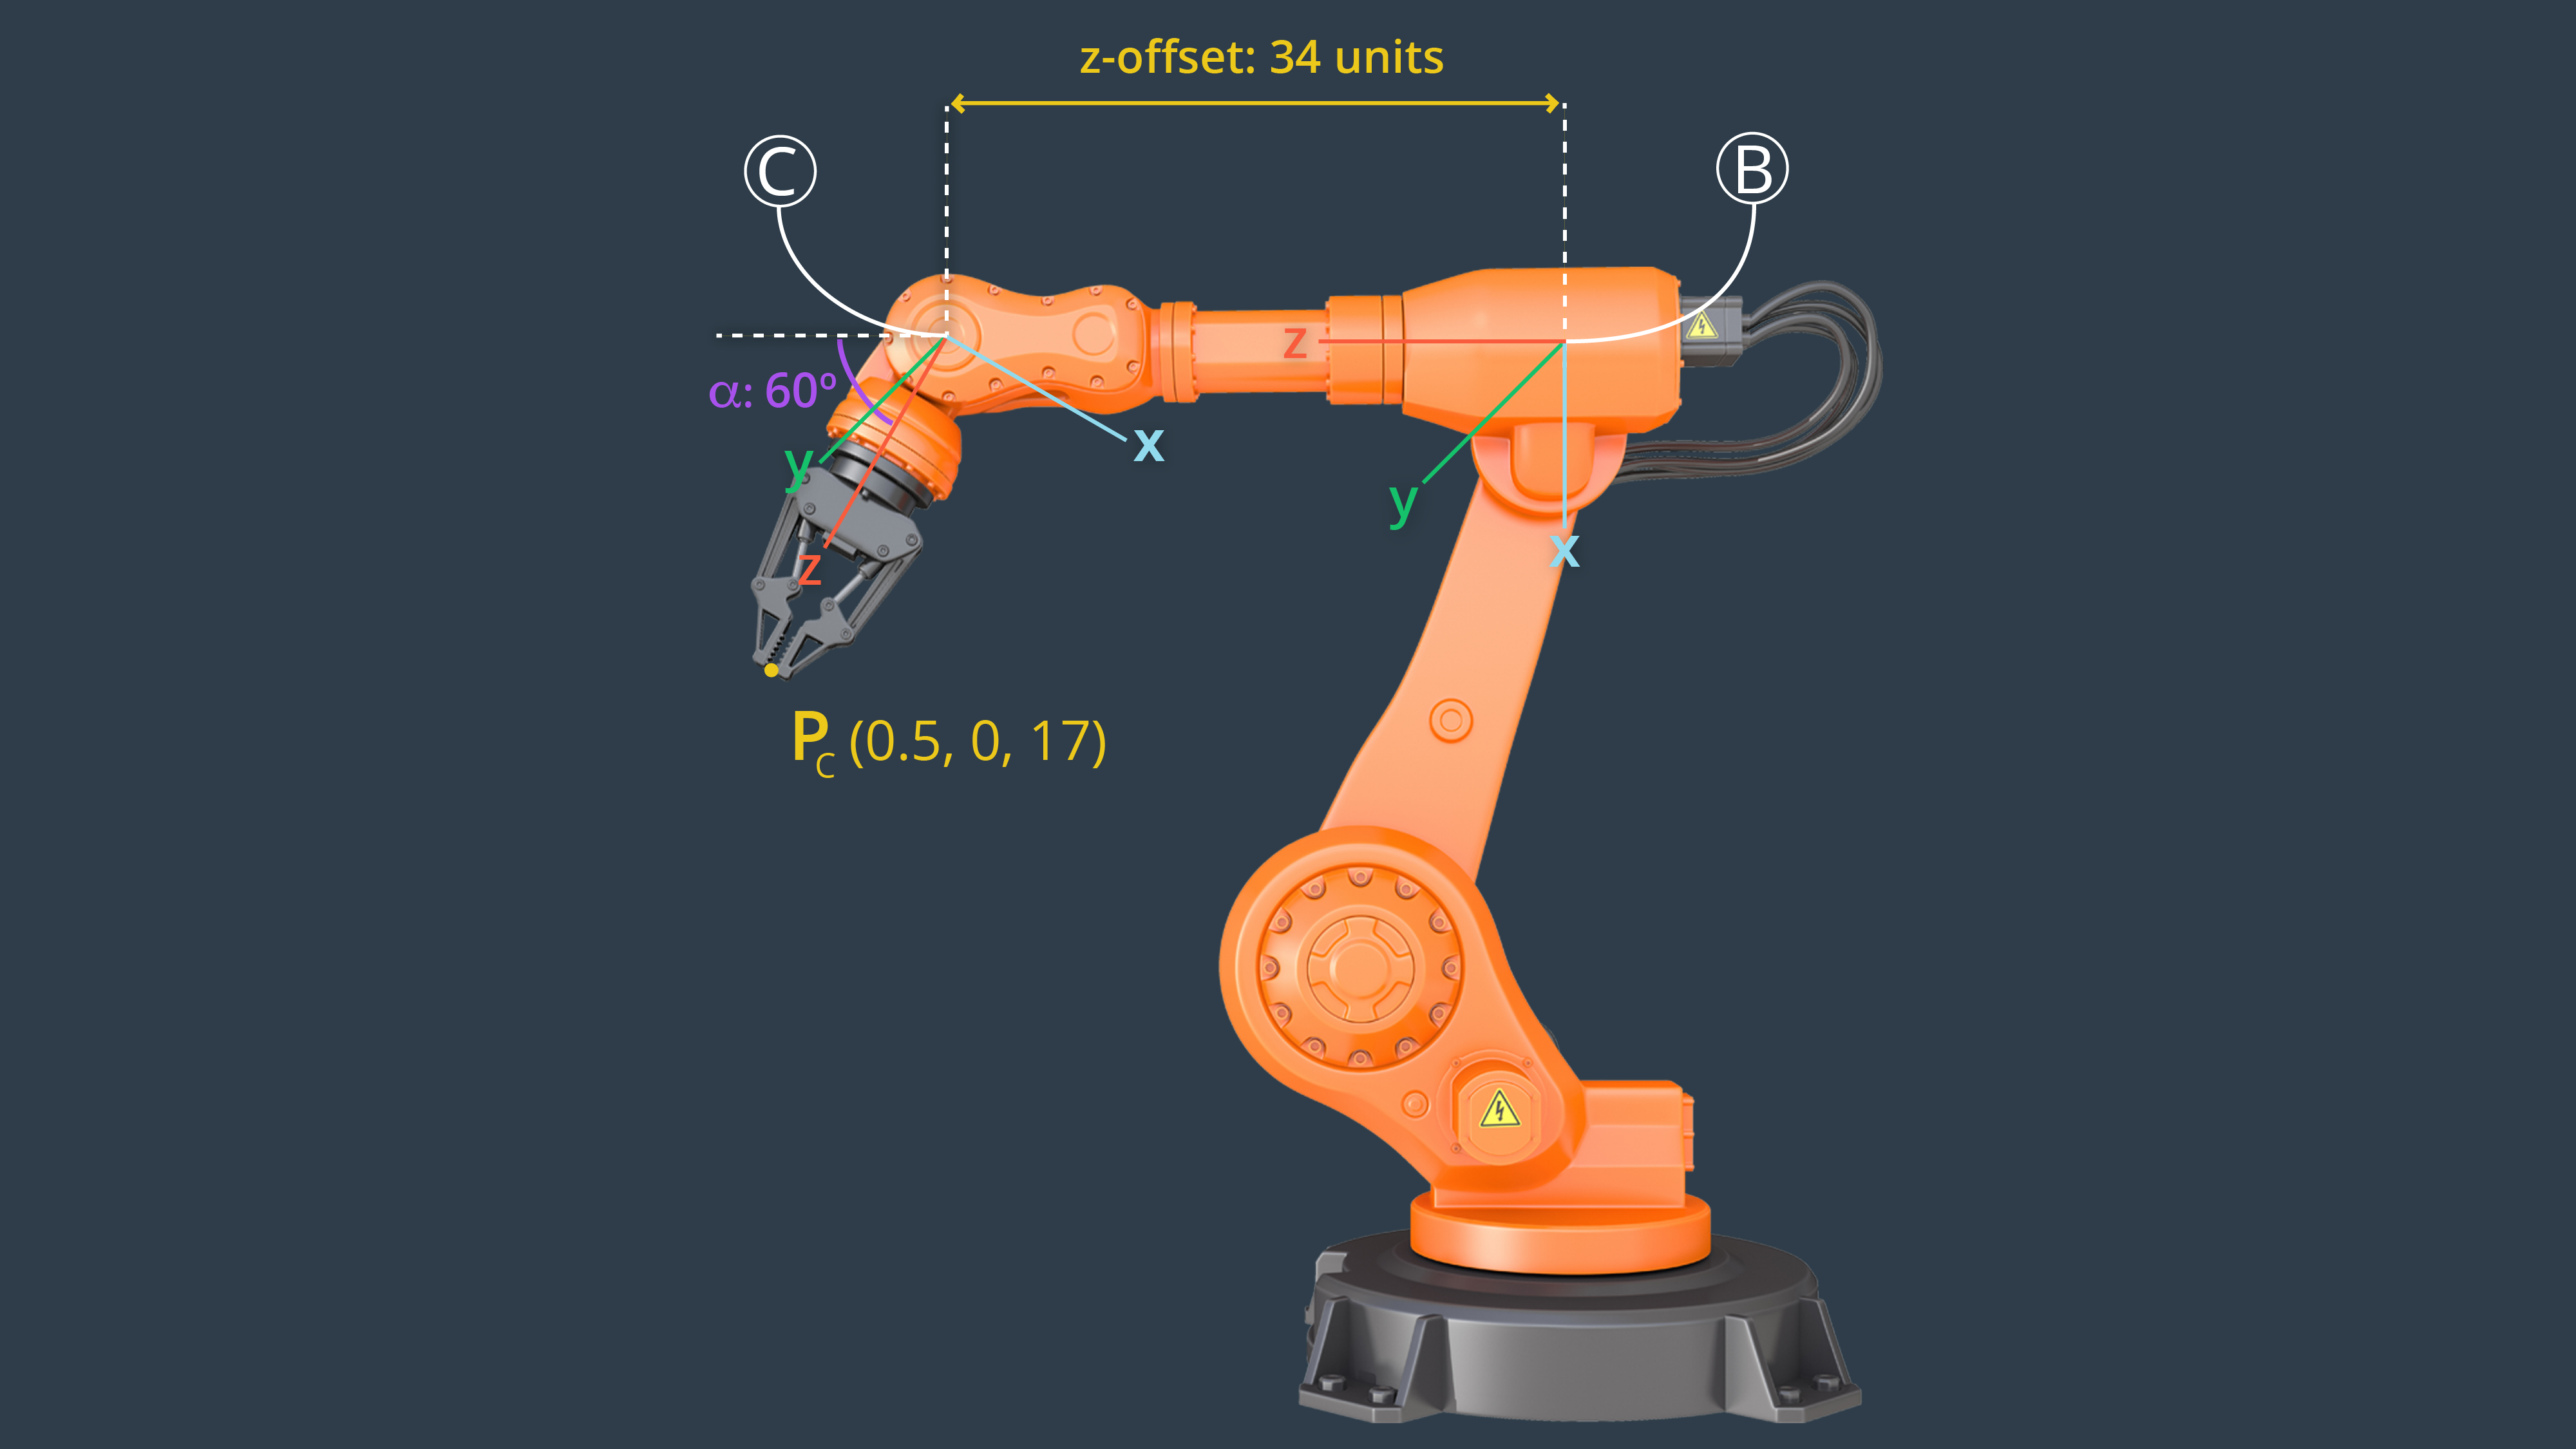
\includegraphics[totalheight=9cm]{imgs/arm-step-1.png}
\end{figure}}
\maketitle
\section{Manipulator: plans and actions}
Fig.~\ref{fig:steps} shows the different steps performed by the simulator for the pick and place of each cylinder.


\begin{figure}[H]
\centering
       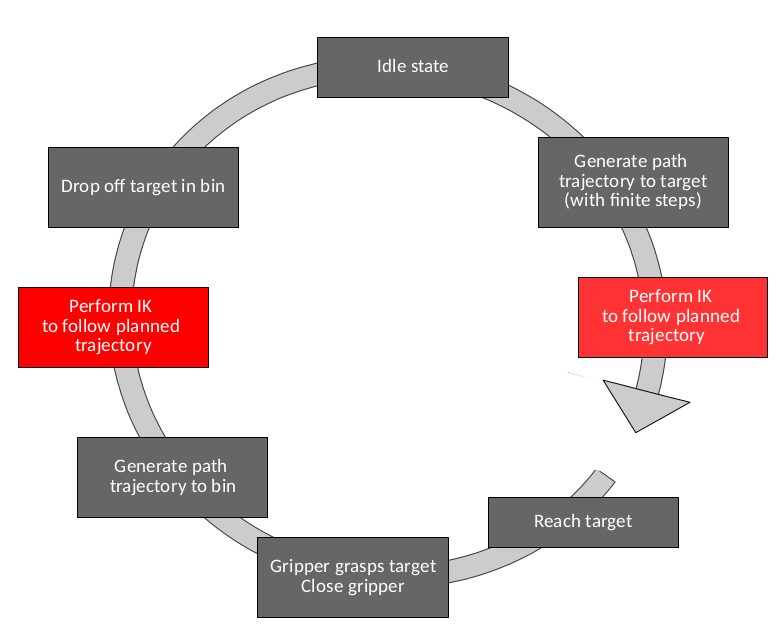
\includegraphics[totalheight=12cm]{imgs/steps.png}
       \caption{Steps performed by the simulator}
       \label{fig:steps}
\end{figure}

When the ROS simulator generates the path trajectory, it provides a set of poses for the Gripper. Our goal is to compute the Inverse Kinematics so that the gripper position and orientation match the position and orientation computed by the planner.

\section{Kinematics Analysis}

\section{Manipulator geometry: reference frames}
In order to determine the modified DH parameter, we need to assign reference frames to each joint according to the DH convention. Fig. \ref{fig:idle_state} shows the joint configuration with the manipulator in the \textit{Idle state} ($i.e$ all joint variables are set to 0).

\begin{figure}[H]
\centering
        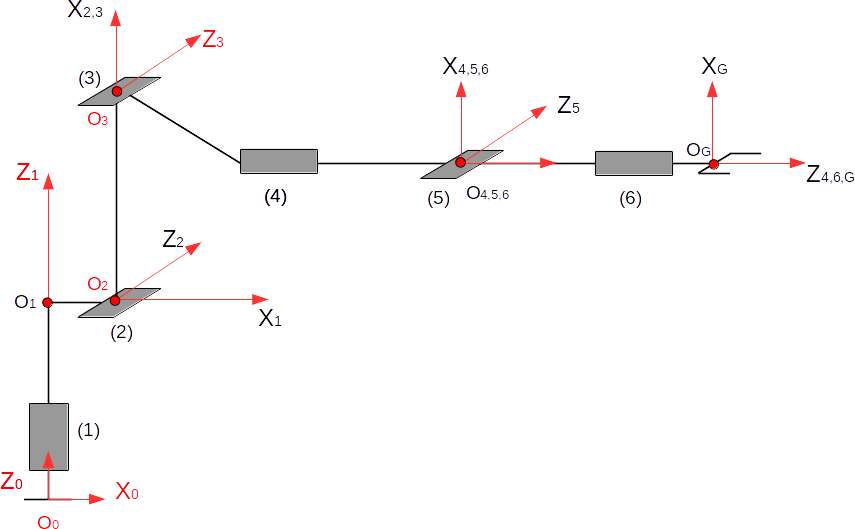
\includegraphics[totalheight=12cm]{imgs/idle_state.png}
        \caption{Initial pose of the manipulator. The joint variables $\theta_i = 0 \ \forall i \in [1, 6]$. The base frame is $(O_0, X_0, Y_0, Z_0)$}
\label{fig:idle_state}
\end{figure}


\section{Modified DH Parameter tables}
The 4 DH parameters are defined as follows:
\begin{itemize}
\item link length: $a_i = [\hat{z}_{i-1}, \hat{z}_i]_{\hat{x}_i}$
\item link twist: $\alpha_i = \left< \hat{z}_{i-1}, \hat{z}_i \right> _{\hat{x}_i}$
\item link offset: $d_i = [\hat{x}_{i-1}, \hat{x}_i]_{\hat{z}_{i-1}}$ 
\item joint offset: $\theta_i = \left< \hat{x}_{i-1}, \hat{x}_i \right> _{\hat{z}_{i-1}}$
\end{itemize}
The notations $[ \ ]$ and $\left< \ \right>$ refer respectively to a distance and an angle, along or about the axis given by the subscript. 

The DH parameters are determined from the \textit{URDF} (\textit{\textbf{kr210.urdf.xacro}}) file and the frame axis attributed according to the DH convention.

\begin{figure}[H]
\centering
        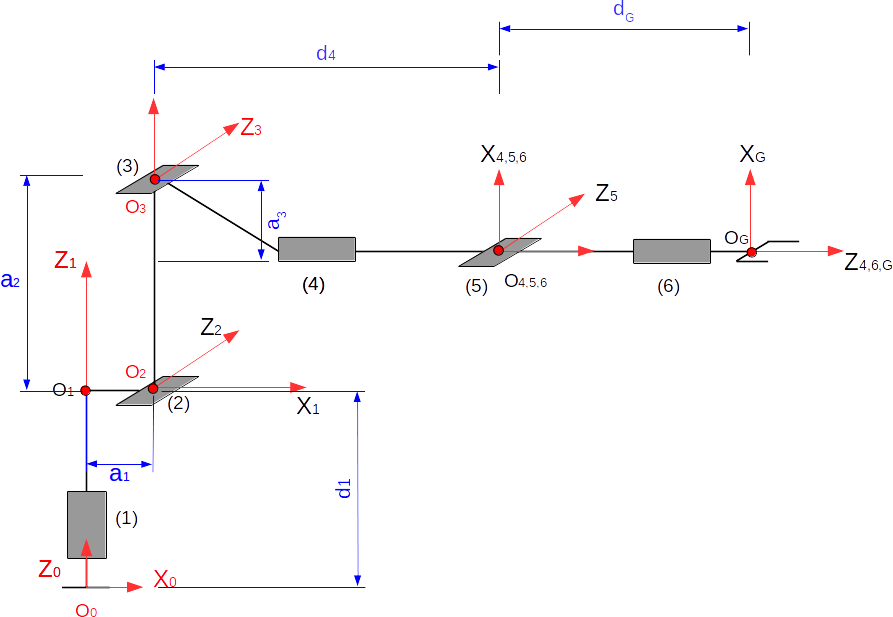
\includegraphics[totalheight=12cm]{imgs/DH_parameters.png}
        \caption{The non-zero DH parameters.}
\end{figure}

Table~\ref{table:urdf} shows the position and orientation of the joint \{$i$\} wrt the joint  \{$i-1$\}, as extracted from the \textit{URDF} file.


\begin{table}[H]
\centering
\begin{tabular}{ | c | c | c | c| c |c|c| }
\hline
 joint & $\Delta x$ & $\Delta y$  & $\Delta z$ & roll & pitch & yaw \\ 
 \hline
1 & 0 & 0 & 0.33 & 0 & 0 & 0 \\  
 \hline
2 & 0.35 & 0 & 0.42 & 0 & 0 & 0 \\  
 \hline
3 & 0 & 0 & 1.25 & 0 & 0 & 0 \\   
 \hline
4 & 0.96 & 0 & -0.054 & 0 & 0 & 0 \\   
 \hline
5 & 0.54 & 0 & 0 & 0 & 0 & 0 \\   
 \hline
6 & 0.193 & 0 & 0 & 0 & 0 & 0 \\  
 \hline
Gripper & 0.11 & 0 & 0 & 0 & 0 & 0 \\  
   \hline 
\end{tabular}
\caption{Relative distances extracted from the file \textit{\textbf{kr210.urdf.xacro}}.}
\label{table:urdf}
\end{table}


In the reference frame, the position of joint \{2\} relative to joint \{1\}  is 0.35m along $\hat{x}$ direction and 0.42 along $\hat{z}$ direction. The later distance corresponds to the distance $[O_1, O_2]$, i.e the link distance $d_1$. Similarly, $d_G$ is the distance $[O_6, O_G] = 0.193 + 0.11$, $i.e$ the $x$ displacement along $\hat{x}$ from joint \{5\} to joint \{6\} added together with the displacement from joint \{6\} to joint \{$G$\} along $\hat{x}$. Similarly, we can use the \textit{URDF} file to determine the non-zero DH parameters $a_i$ and $d_i$ (Table~\ref{table:dh_table}).


\begin{table}[H]
\centering
\begin{tabular}{ | c | c | c | c| c | }
\hline
 link $i$ & $\alpha_{i-1}$ & $a_{i-1}$  & $d_i$ & $\theta_i$ \\ 
 \hline
1 & 0 & 0 & 0.75 & $q1$ \\  
 \hline
2 & $-\pi/2$ & 0.35 & 0 & $q2 - \frac{\pi}{2}$ \\
 \hline
3 & 0 & 1.25 & 0 & $q3$ \\ 
 \hline
4 & $-\pi/2$ & -0.054 & 1.50 & $q4$ \\ 
 \hline
5 & $\pi/2$ & 0 & 0 & $q5$ \\ 
 \hline
6 & $-\pi/2$ & 0 & 0 & $q6$ \\ 
 \hline
G & 0 & 0 & $dG = 0.303$ & 0 \\ 
   \hline 
\end{tabular}
\caption{Modified DH Parameter table}
\label{table:dh_table}
\end{table}

\section{Homogeneous Transforms}
\subsection{General form of the homogeneous Transform}
The homogeneous transform $T_{i-1} ^{i}$ is an expression of the orientation and position of joint \{$i$\} with respect to joint \{$i-1$\}. The homogeneous transform is composed of 2 rotations($\alpha$ and $\theta$) and 2 translations ($a$ and $d$):

\begin{equation}
\label{eqTransf}
_{i-1} ^{i} T  = \left( \begin{matrix} \text{cos} \theta_i & -\text{sin} \theta_i & 0 & a_{i-1} \\
\text{sin} \theta_i \text{\ cos} \alpha_{i-1} & \text{cos} \theta_i \text{\ cos} \alpha_{i-1}& -\text{\ sin} \alpha_{i-1} & -d_i \text{\ sin} \alpha_{i-1} \\
\text{sin} \theta_i \text{\ sin} \alpha_{i-1} & \text{cos} \theta_i \text{\ sin} \alpha_{i-1} & \text{cos} \alpha_{i-1} & d_i \text{\ cos} \alpha_{i-1} \\
0 & 0 & 0 & 1
\end{matrix} \right)
\end{equation}

In the code \textit{IK\_server.py}, we create a function that generates the general form of the Homogeneous transform (Line 23-30 )

\subsection{Homogenemous Transform for each frame transition}
Using the modified DH parameter table (Table~\ref{table:dh_table}) and Eq. \ref{eqTransf}, we determine the Homogeneous transform for each transition:

\begin{itemize}
\item $_1 ^0 T = \left( \begin{matrix} \text{cos}(q_1) & -\text{sin}(q_1) & 0 & 0 \\
\text{sin}(q_1) & \text{cos}(q_1) & 0 & 0 \\
0 & 0 & 1 & 0.75 \\
0 & 0 & 0 & 1
 \end{matrix} \right)$
 
\item $_2 ^1 T = \left( \begin{matrix} \text{sin}(q_2) & -\text{cos}(q_2) & 0 & 0.35 \\
0 & 0 & 1 & 0 \\
\text{cos}(q_2) & -\text{sin}(q_2) & 0 & 0 \\
0 & 0 & 0 & 1
 \end{matrix} \right)$
 
\item $_3 ^2 T = \left( \begin{matrix} \text{cos}(q_3) & -\text{sin}(q_3) & 0 & 1.25 \\
\text{sin}(q_3) & \text{cos}(q_3) & 0 & 0 \\
0 & 0 & 1 & 0 \\
0 & 0 & 0 & 1
 \end{matrix} \right)$
 
\item $_1 ^0 T = \left( \begin{matrix} \text{cos}(q_4) & -\text{sin}(q_4) & 0 & -0.054 \\
0 & 0 & 1 & 1.5 \\
-\text{sin}(q_4) & -\text{cos}(q_4) & 0 & 0 \\
0 & 0 & 0 & 1
 \end{matrix} \right)$
 
\item $_5 ^4 T = \left( \begin{matrix} \text{cos}(q_5) & -\text{sin}(q_5) & 0 & 0 \\
0 & 0 & -1 & 0 \\
\text{sin}(q_5) & \text{cos}(q_5) & 0 & 0 \\
0 & 0 & 0 & 1
 \end{matrix} \right)$

\item $_6 ^5 T = \left( \begin{matrix} \text{cos}(q_6) & -\text{sin}(q_6) & 0 & 0 \\
0 & 0 & -1 & 0 \\
\text{sin}(q6) & \text{cos}(q_6) & 0 & 0 \\
0 & 0 & 0 & 1
 \end{matrix} \right)$

\item $_G ^6 T = \left( \begin{matrix} 1 & 0 & 0 & 0 \\
0 & 1 & 0 & 0 \\
0 & 0 & 1 & 0.303 \\
0 & 0 & 0 & 1
 \end{matrix} \right)$
\end{itemize}

Note that the last homogeneous transform ($_G ^6 T$) is only a translation of the frame \{6\} (no rotation).

The Homogeneous Transform matrix from base link to gripper link is a post-multiplication of the individual homogeneous transformation matrix:

\begin{align}
_G ^0 T = _0 ^1 T \  _1 ^2 T \ _2 ^3 T \ _3 ^4 T \ _4 ^5 T \ _5 ^6 T \ _6 ^G T
\end{align}

In \text{IK\_server.py}, those matrices are defined line 99-126.
\begin{figure}[H]
\centering
        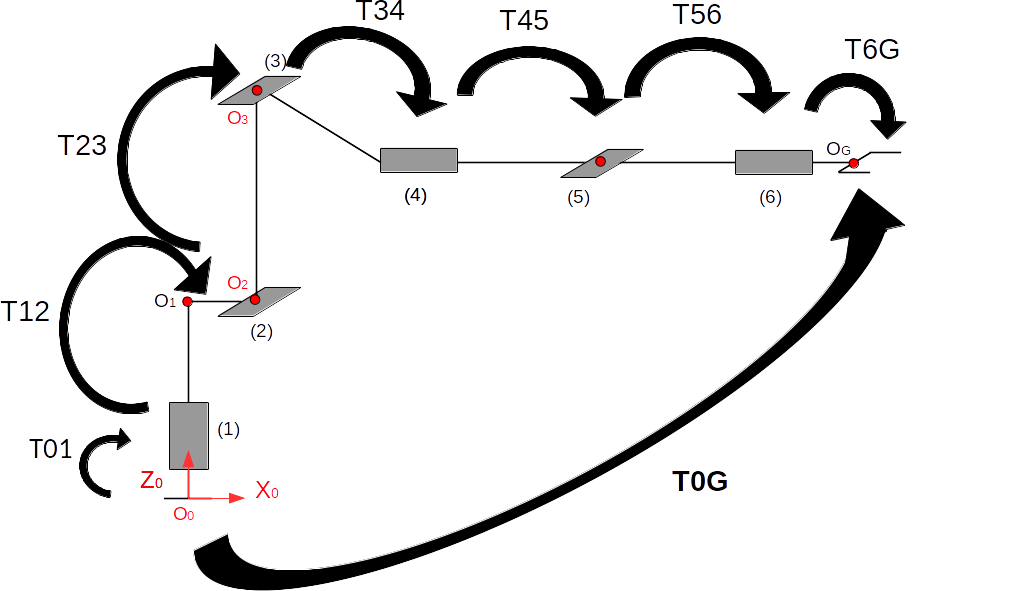
\includegraphics[totalheight=12cm]{imgs/transform.png}
        \caption{The individual homogeneous transforms and the complete homogeneous transform between the base frame and the gripper frame.}
\end{figure}

\section{Inverse Kinematics}
The last 3 joints (namely joint 4, 5 and 6) defines a spherical wrist: they are revolute joints with their axis intersecting at a single point (origin $O_5$). This point is the wrist center $WC$. Using the position of the wrist center, the Inverse Kinematics can be decoupled into a position and orientation problem.

In the next sections, we calculate the cartesian coordinates of $WC$ wrt the base frame, and determine the joint variables.

\subsection{Position of the wrist center}
From Fig.~\ref{fig:fig_wc}, we have:
\begin{align}
^0 r_{C} & \equiv ^0 r_G - d_G \ \hat{z}_G 
\end{align}

where $^0 r_C$ gives the position of the wrist center wrt the base frame, $^0 r_{0G}$ is the vector from the origin to the wrist center wrt to the base frame, and $d_G$ is the distance from the origin of the Gripper frame to the wrist center along $\hat{z}_G$. $\hat{z}_G$ can be expressed in the base reference frame by computing its projection onto the 3 axis $(X_0, Y_0, Z_0)$, which is in fact the last column of the rotation matrix $_G ^0 R$. Hence:
\begin{align}
^0 r_{C} = \left[ \begin{matrix} w_x \\ w_y \\ w_z \end{matrix} \right] ^0 r_G - d_G \ _G ^0 R \left[\begin{matrix} 0 \\ 0 \\ 1 \end{matrix} \right] 
\end{align}


\begin{figure}[H]
\centering
        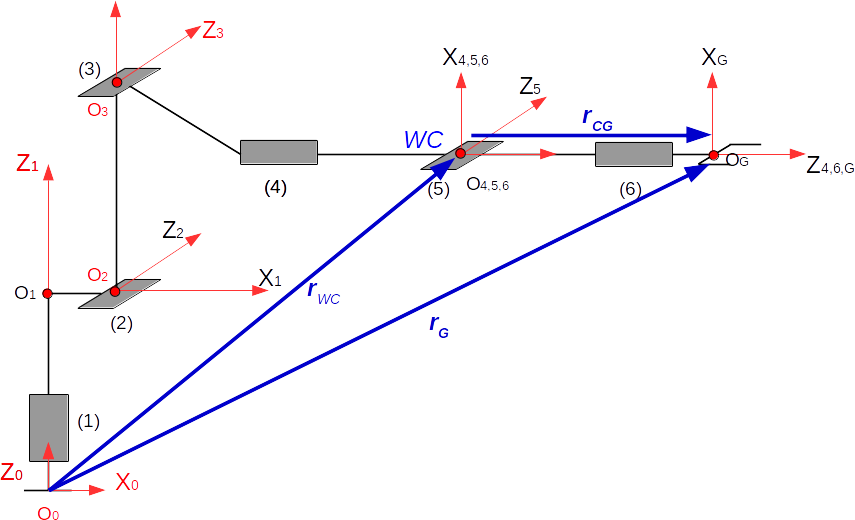
\includegraphics[totalheight=12cm]{imgs/wrist_center.png}
        \caption{Wrist center position with the manipulator in Idle mode configuration.}
        \label{fig:fig_wc}
\end{figure}


\subsection{Transformation Matrix between the gripper frame and the base frame}
The path planner provides 6 parameters: the position and the orientation of the gripper wrt to the base frame: ($p_x, p_y, p_z, roll, pitch, yaw)$.  We can build the transformation matrix (in the DH frame): $_G ^0T$, by determining the rotation matrix $_G ^0R$ from the roll, yaw and pitch. In addition, we need to apply a correction to account for the misalignment between the gripper frame in the urdf file and the gripper frame according to the DH convention.

\begin{enumerate}
\item Compute the total rotation matrix $^{urdf}R_G$, in the \textit{"urdf frame"} using the individual rotation matrices with roll ($r$), pitch ($p$), yaw $y$  angles:
\begin{align}
R_x = \left( \begin{matrix} 1 & 0 & 0 \\
0 & \text{cos}(r) & -\text{sin}(r) \\
0 & \text{sin}(r) & \text{cos}(r) \end{matrix}\right) & 
R_y = \left( \begin{matrix} \text{cos}(p) & 0 & \text{sin}(p) \\
0 & 1 & 0 \\
-\text{sin}(p) & 0 &  \text{cos}(p) \end{matrix}\right) &
R_z = \left( \begin{matrix} \text{cos}(y) & -\text{sin}(y) & 0 \\
\text{sin}(y) & \text{cos} (y) & 0 \\
0 & 0 & 1 \end{matrix}\right)
\end{align}

Hence:
\begin{align}
^{urdf} R_{G} = R_z \ R_y \ R_x
\end{align}


\item Apply rotation correction. From Fig.~\ref{fig:urdf_dh}, the gripper axis according to the urdf file can be aligned with the gripper axis from the DH convention by applying 2 intrinsic rotations: a rotation  of $\pi$ about $\hat{z}_u$ axis, and a rotation of $-\pi/2$ about $\hat{y}_u$ $R_{z_{u}}(\pi) R_{y_{u}}(-\pi/2)$. Hence the orientation of the gripper wrt to the base frame and within the DH framework is:

\begin{align}
_G ^0 R = \ \left( ^{urdf} R_{G} \right) * R_z(\pi) * R_y(-\pi/2)
\end{align}

\begin{figure}[H]
\centering
        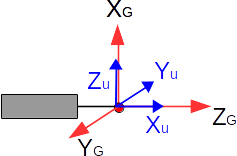
\includegraphics[totalheight=6cm]{imgs/urdf-dh.png}
        \caption{$(X_G, Y_G, Z_G)$ are the axis of the gripper frame according to the DH convention (red), and $(X_u, Y_u, Z_u)$ are the axis of the gripper frame as in the urdf file (blue).}
        \label{fig:urdf_dh}
\end{figure}

\item Homogeneous transform matrix:

\begin{equation}
_G ^0 T = \left[ \begin{array}{c;{2pt/2pt}c} _G ^0 R & p \\ \hdashline[2pt/2pt]
0 0 0 & 1 \end{array} \right]  \text{\ \ \ \ \ where\ } p=\left[ \begin{matrix} p_x \\ p_y \\ p_z \end{matrix} \right]
\end{equation}


\end{enumerate}

In \textit{IK\_server.py}, the orientation matrix and position vector of the Gripper is computed from line 148-166. 

\subsection{Determine Joint angles}

\subsubsection{Joint angle 1: $q1 = \left< \hat{x}_0, \hat{x}_1 \right> _{z_0} $}
We can calculate $q1$ from the coordinates of the wrist center (From Fig ~\ref{fig:q1}.

\begin{align}
q1 = atan2 \left(\frac{w_y}{w_x} \right)
\end{align}

\begin{figure}[H]
\centering
        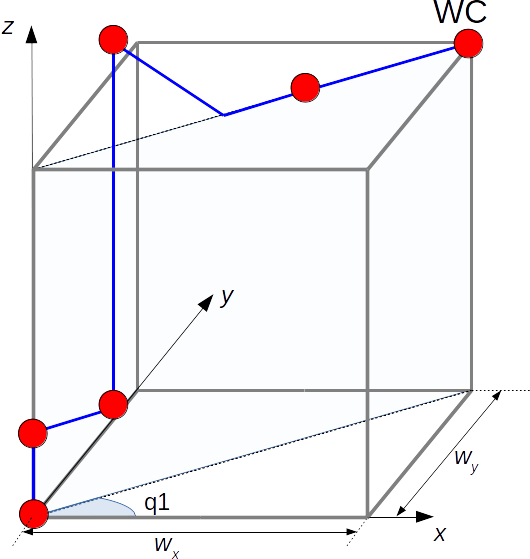
\includegraphics[totalheight=7cm]{imgs/q1.png}
        \caption{Joint 1 is rotated by angle $q1$. ($w_x, w_y$) are the coordinates of the wrist center wrt to the base reference frame.}
        \label{fig:q1}
\end{figure}

According to the $URDF$ file, the joint 1 angles are limited to the  range $-185 < q1 < 185$.

\subsubsection{Joint angle 2: $q2 = \left< \hat{x}_1, \hat{x}_2 \right> _{z_1} $}

$q2$ is given by:
\begin{equation}
\label{eq:eq10}
q2 = \pi/2 - a - a'
\end{equation}

\begin{figure}[H]
\label{fig:figq2}
\begin{multicols}{2}
    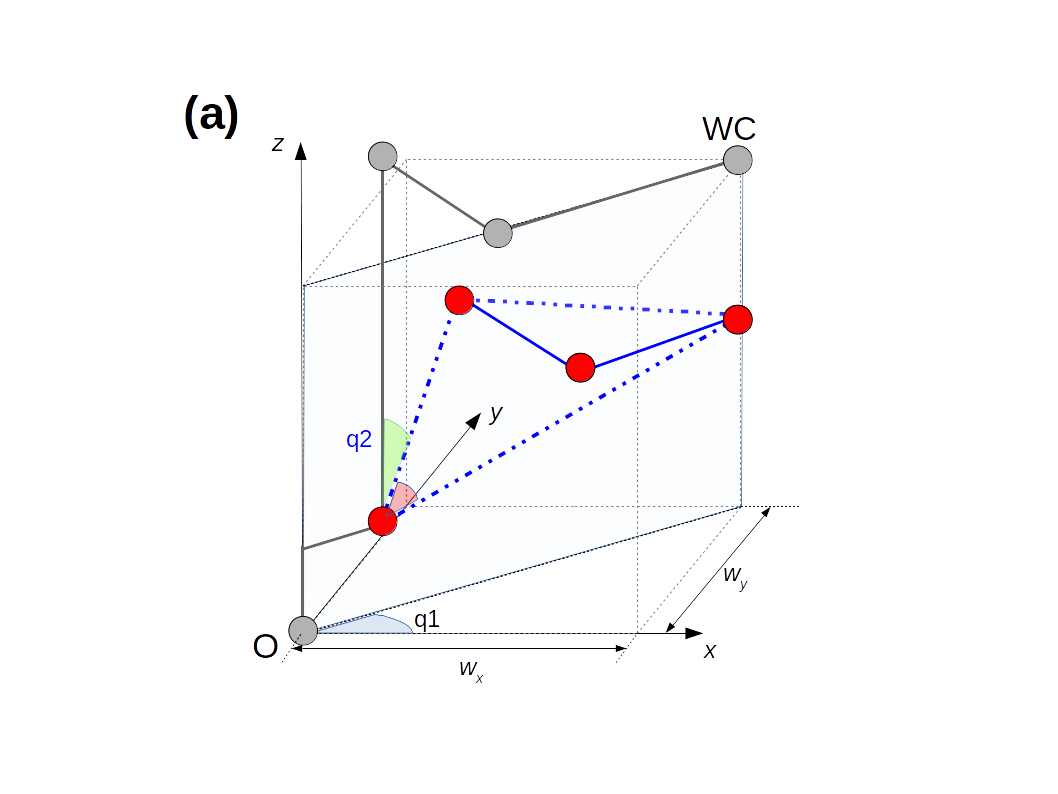
\includegraphics[width=10cm]{imgs/q2_1.png}\par 
    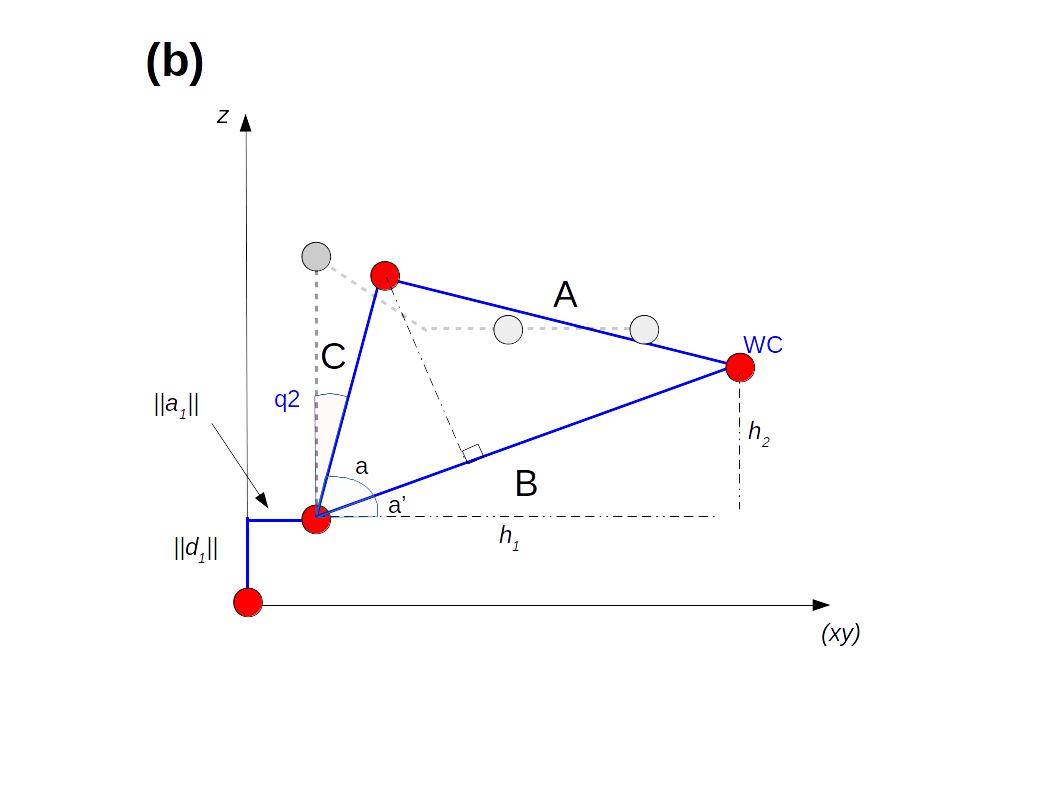
\includegraphics[width=10cm]{imgs/q2_2.png}\par 
\end{multicols}
\caption{a) Joints configuration when the joint \{2\} is rotated by an angle $q2$. The grey line/dots shows the manipulator geometry when in idle mode. b) Visualization of the joints and links in the plane (Oz, OWC)}

\end{figure}

Using cosine law, we can determine the angle $a$:

\begin{align}
A^2 &= B^2 + C^2 - 2BC cos(a)  \\
\Rightarrow cos(a) = \frac{B^2 + C^2 - A^2}{2 B \ C} \ \ &\text{and} \  \ sin(a) = \sqrt{(1- cos^2 a)}
\end{align}

Hence:

\begin{equation} 
\label{eq:eq14}
a = atan2 \left( \frac{1 - cos^2 a}{cos(a)} \right)
\end{equation}

The angle $a$ can take either a positive or a negative value depending on the sign of $sin(a)$. This would result in a elbow up/down configuration.


From Fig. Fig. 8b, $h$ is given by:
\begin{align}
h^2  &=  x_c ^2 + y_c ^2  \ \ \Rightarrow \ \ h= \sqrt{x_c ^2 + y_c ^2} \\
h_1 + a_2 &= \sqrt{x_c ^2 + y_c ^2} \ \ \Rightarrow \ \ h_1 = \sqrt{x_c ^2 + y_c ^2} - a_2 \\
\ \ \text{and} h2  &=  z_c - d_1
\end{align}


Hence:
\begin{align} 
\label{eq:eq21}
a' &= atan2\left( \frac{h2}{h1} \right) \\
 &= atan2 \left( \frac{z_c - d_1}{ \sqrt{x_c ^2 + y_c ^2} - a_2 } \right)
\end{align}


Substituting Equation Eq. \ref{eq:eq14}  and Eq. \ref{eq:eq21} in Eq. \ref{eq:eq10}, we obtain:

\begin{equation}
q2 = \frac{\pi}{2} - atan2\left( \frac{sin(a)}{cos(a)} \right) - atan2 \left( \frac{z_c - d_1}{ \sqrt{x_c ^2 + y_c ^2} - a_2 } \right)
\end{equation}

According to the $urdf$ file, the joint angle has a upper and a lower safe limit  of -45deg and +85deg respectively. We will therefore clip $q2$ to that range of angles.  

\subsubsection{Joint angle 3: $q3 = \left< \hat{x}_2, \hat{x}_3 \right> _{z_2} $}

\begin{figure}[H]
\centering
        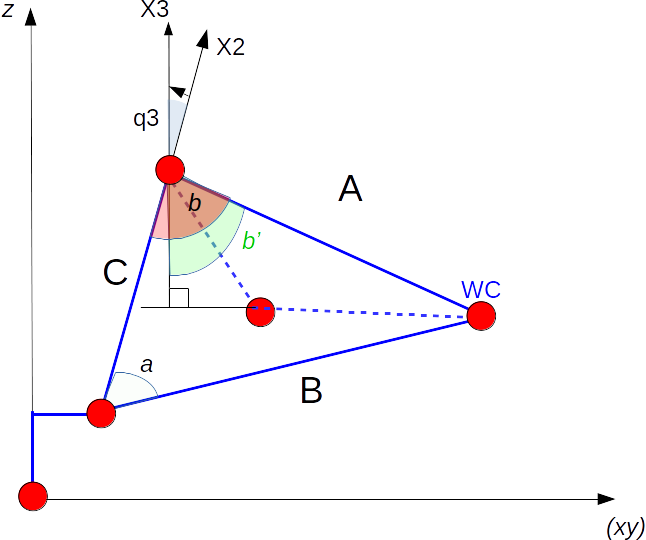
\includegraphics[totalheight=7cm]{imgs/q3.png}
        \caption{Angle $q3$}
        \label{fig:q1}
\end{figure}

\begin{align}
q3 &= - (b - b') \\
&= - \left( b - atan2 \left( \frac{d_4}{a_3} \right) \right)
\end{align}

From the cosine law, we get:
\begin{align}
cos(b) &= \frac{A^2 + C^2 - B^2}{2 AC} \\
sin^2(b) &= 1 - cos^2(b)
\end{align}

Hence:

\begin{align}
b = atan2\left( \frac{sin(b)}{cos(b)}\right) 
\end{align}
Finally, $q3$ is:
\begin{align}
q3 = - atan2\left( \frac{sin(b)}{cos(b)}\right)  + atan2 \left( \frac{d_4}{a_3} \right)
\end{align}
The angle will be cliped to the range [-210, 65] deg.



\subsubsection{Joint angle 4, 5 and 6}
The last 3 joint angles are determined using the rotation matrix $_i ^{i-1} R$:

\begin{equation}
_G ^0 R = _1 ^ 0 R \ * \ _2 ^ 1 R * \ _3 ^ 2 R * \ _4 ^ 3 R * \ _5 ^ 4 R * \ _6 ^ 5 R * \ _G ^ 6 R 
\end{equation}
The transformation from frame \{6\} to frame \{G\} is a simple translation so $\ _G ^ 6 R = I$.
Previously, w determined $q1$, $q2$ and $q3$, therefore $ _3 ^0 R = _1 ^ 0 R(q1) \ * \ _2 ^ 1 R(q2) * \ _3 ^ 2 R(q3)$ can be computed. Hence:

\begin{equation}
_G ^0 R =  _3 ^0 R(q1, q2, q3) \ * \ _6 ^3 R(q4,q5,q6)
\end{equation}
and results in:

\begin{equation}
_6 ^3 R(q4,q5,q6) =  \left( _3 ^0 R(q1, q2, q3) ^{\intercal} \right) \ * \ \left( _G ^0  R(r, p, y) \right)
\label{eq:37}
\end{equation}

The general expression of the rotation part of the transformation matrix is:

\begin{equation}
_{i} ^{i-1} R = \left[ \begin{matrix} cos(q_i) & -sin(q_i) & 0 \\
sin(q_i) \ cos(\alpha_{i-1})  & cos(q_i) cos(\alpha_{i-1}) & -sin(\alpha_{i-1}) \\
sin(q_{i}) \ sin(\alpha_{i-1}) & cos(q_i) \ sin(\alpha_{i-1}) & cos(\alpha_{i-1}  \end{matrix}\right]
\label{eq:38}
\end{equation}

From the DH parameter table and Eq. \ref{eq:38}, we estimate $_4 ^3R$, $_5 ^4R$ and $_6 ^5R$:

\begin{align}
\label{eq:39}
_4 ^3 R = \left( \begin{matrix} cos(q4) & -sin(q4) & 0 \\
0 & 0 & -1 \\
-sin(q4) & -cos(q4) & 0 \end{matrix}\right) & 
_5 ^4 R = \left( \begin{matrix} cos(q5) & -sin(q5) & 0 \\
0 & 0 & -1 \\
sin(q5) & cos(q5) & 0 \end{matrix}\right) & 
_6 ^5 R = \left( \begin{matrix} cos(q6) & -sin(q6) & 0 \\
0 & 0 & -1 \\
-sin(q6) & -cos(q6) & 0 \end{matrix}\right)
\end{align}

From Eq. \ref{eq:39}, the rotation matrix $_6 ^3 R$ is computed:
 	
\begin{equation}
_{6} ^{3} R = \left[ \begin{matrix} c(q_4)c(q5)c(q6) -s(q4)s(q5) & -c(q4)c(q5)s(q6)-c(q5)s(q6)-c(q5)s(q4) & c(q4)s(q5) \\
s(q5) c(q6)  & -s(q5)s(q6) & c(q5) \\
-s(q4)c(q5)c(q6)-c(q4)s(q5) & s(q4)c(q5)s(q6)-c(q4)c(q5)  & -s(q4)s(q5)  \end{matrix}\right]
\label{eq:38}
\end{equation}

$_G ^0 R(r,p,y)$ is the orientation of the Gripper in the reference frame O. It includes the roll, pitch, yaw rotation and a correction rotatiton term to align the $urdf$ frame with the DH convention frame. By comparing Eq. \ref{eq:39} and Eq. \ref{eq:37}, the joint angles $q4, q5, q6$ are determined:

\begin{align}
q4 &= atan2\left( -\frac{-s(q4)s(q5)}{c(q4)s(q5)}\right) = atan2 \left(-\frac{R[0,2]}{R[2,2]} \right) \\
q5 &=  atan2\left( \frac{[(s(q5)c(q6))^2 + s(q5)s(q6)]^{0.5}}{c(q5)}\right) = atan2 \left(\frac{[R[1,0]^2 + R[1,1]^2]^{0.5} }{R[1,2]} \right) \\
q6 &=  atan2\left(- \frac{-s(q5)s(q6)}{s(q5)c(q6)}\right) = atan2 \left(-\frac{R[1,1] }{R[1,0]} \right)
\end{align}


where $R = \left( _3 ^0 R(q1, q2, q3) ^{\intercal} \right) \ * \ \left( _G ^0  R(r, p, y) \right)$

Each of the joint angles $q4$, $q5$ and $q6$ are clipped to the angle range given in the $urdf$ file: $q_4$-limit = [-350, 350], $q5$-limit=[-125, 125], $q6$-limit=[-350,250].
Note taht $q5$ has multiple solution:positive or negative value.
\section{Comments}
I have implemented all of the parts detailed in this report. However, I have found some bugs that I have not been able to resolved:

\begin{itemize}
\item if I clip all the joint angles to their respective values, there is no improvement, in fact no difference, in the behaviour of the manipulator.

\item If $q2$ and $q3$ are clipped to their respective safe angle limit, the gripper consistently fails to grap the cylinder. That is to say that the gripper fingers would be placed appropriately around the cylinder, but after clicking [NEXT] to retrieve, the gripper would fail to carry the cylinder off the shelf.

\item I also tried to prevent hectic behaviour of the manipulator by comparing current and previous angles. Because some joint angles can have multiple solutions, it is likely that 2 consecutives angle of a joint coudl have solutions that are in 2 different quadrants. To prevent this behaviour, I implemented a function \textit{validate()}. This function takes the current theta value and the old theta value, and select the solution that is in the same quadrant as the previous angle value.

\end{itemize}

\end{document}